%%%%%%%%%%%%%%%%%%%%%%%%%%%%%%%%%%%%%%%%%
% Beamer Presentation
% LaTeX Template
% Version 1.0 (10/11/12)
%
% This template has been downloaded from:
% http://www.LaTeXTemplates.com
%
% License:
% CC BY-NC-SA 3.0 (http://creativecommons.org/licenses/by-nc-sa/3.0/)
%
%%%%%%%%%%%%%%%%%%%%%%%%%%%%%%%%%%%%%%%%%

%----------------------------------------------------------------------------------------
%	PACKAGES AND THEMES
%----------------------------------------------------------------------------------------

\documentclass[t]{beamer}

\mode<presentation> {

% The Beamer class comes with a number of default slide themes
% which change the colors and layouts of slides. Below this is a list
% of all the themes, uncomment each in turn to see what they look like.

%\usetheme{default}
%\usetheme{AnnArbor}
%\usetheme{Antibes}
%\usetheme{Bergen}
%\usetheme{Berkeley}
%\usetheme{Berlin}	% *
%\usetheme{Boadilla}
%\usetheme{CambridgeUS}
%\usetheme{Copenhagen}	
%\usetheme{Darmstadt}
%\usetheme{Dresden}
%\usetheme{Frankfurt}
%\usetheme{Goettingen}	% SO right
%\usetheme{Hannover}		% SO left
%\usetheme{Ilmenau}
%\usetheme{JuanLesPins}
%\usetheme{Luebeck}		
%\usetheme{Madrid}
%\usetheme{Malmoe}
%\usetheme{Marburg}
%\usetheme{Montpellier}
%\usetheme{PaloAlto}
%\usetheme{Pittsburgh}	% simple
%\usetheme{Rochester}
%\usetheme{Singapore}
%\usetheme{Szeged}
\usetheme{Warsaw}		% p2p

% As well as themes, the Beamer class has a number of color themes
% for any slide theme. Uncomment each of these in turn to see how it
% changes the colors of your current slide theme.

%\usecolortheme{albatross}
%\usecolortheme{beaver}
%\usecolortheme{beetle}
%\usecolortheme{crane}
%\usecolortheme{dolphin}
%\usecolortheme{dove}
%\usecolortheme{fly}
%\usecolortheme{lily}
%\usecolortheme{orchid}
%\usecolortheme{rose}
%\usecolortheme{seagull}
%\usecolortheme{seahorse}
%\usecolortheme{whale}
%\usecolortheme{wolverine}
\usecolortheme{spruce}


%\setbeamertemplate{footline} % To remove the footer line in all slides uncomment this line
%\setbeamertemplate{footline}[page number] % To replace the footer line in all slides with a simple slide count uncomment this line

%\setbeamertemplate{navigation symbols}{} % To remove the navigation symbols from the bottom of all slides uncomment this line
}
\usepackage{multicol}
\usepackage{caption}
\usepackage{pgfgantt}
\usepackage{graphicx} % Allows including images
\usepackage{booktabs} % Allows the use of \toprule, \midrule and \bottomrule in tables

% LOGO

\beamertemplatenavigationsymbolsempty
\setbeamertemplate{footline}[frame number]
\usepackage{tikz}
\usepackage{pgf}
\logo{
\includegraphics[height=1.5cm]{logo.pdf}}
\newcommand{\nologo}{\setbeamertemplate{logo}{}}

\newcommand{\myquote}[2]{\begin{exampleblock}{}{\large ``#1''}\vskip5mm\hspace*\fill{\small--- #2}\end{exampleblock}}
%----------------------------------------------------------------------------------------
%	TITLE PAGE
%----------------------------------------------------------------------------------------

\title[Hyper-linked Communications]{Hyper-linked Communications: WebRTC enabled
asynchronous collaboration} % The short title appears at the bottom of every slide, the full title is only on the title page

\author{Henrique Rocha} % Your name
\institute[IST] % Your institution as it will appear on the bottom of every slide, may be shorthand to save space
{
Instituto Superior Técnico \\
Universidade de Lisboa \\ % Your institution for the title page
\medskip
\textit{henrique.rocha@tecnico.ulisboa.pt} % Your email address
}
\date{\today} % Date, can be changed to a custom date

\begin{document}
{
%\nologo
\begin{frame}
\titlepage % Print the title page as the first slide
\end{frame}
}

\begin{frame}[t,allowframebreaks]
\frametitle{Overview} 
\tableofcontents[part=1]
\framebreak
\tableofcontents[part=2]
\end{frame}

%----------------------------------------------------------------------------------------
%	PRESENTATION SLIDES
%----------------------------------------------------------------------------------------

%------------------------------------------------
\part{1}
\section{Introduction}\label{intro}

\begin{frame}[t,shrink]
\frametitle{Related Work} 
\tableofcontents[part=1,currentsection,hideothersubsections]
\tableofcontents[part=2,currentsection,hideothersubsections]
\end{frame}

	\subsection{Context}   % English
		\begin{frame}[c]
		\frametitle{Context}
		Written communication could never replace face to face communication.

		\myquote{No computer in our lifetimes will ever rival a human voice's capacity to conveying rich and complex social and emotional meaning}{Geddes, Martin}

		Today, we can achieve more.
		\end{frame}

	\subsection{Problem Statement} % English
  		\begin{frame}[c]
		\frametitle{Problem Statement}
		Real-time communication applications can make a difference on business, education and health sectors.

		\vfill

		An application that provides a way to remember our past communications would be a strong tool.
		\end{frame}

	\subsection{Thesis Goals} % English
  		\begin{frame}[c]
		\frametitle{Thesis Goals}
		Development of an application that applies the hypermedia concepts.

		\vfill

		Use only standard technologies like JavaScript, WebRTC, HTML5 and CSS3.

		\vfill

		Test the application with real users, unitary tests and benchmarks
		\end{frame}


\section{Related Work}\label{related}

\begin{frame}[t,shrink]
\frametitle{Related Work} 
\tableofcontents[part=1,currentsection,hideothersubsections]
\tableofcontents[part=2,currentsection,hideothersubsections]
\end{frame}

	\subsection{Early days of the Internet and its remaining flaws}\label{early}


  		\begin{frame}[c]
		\frametitle{Early days of the Internet and its remaining flaws}
		\begin{itemize}
		\item IPv4 Address Exhaustion
		\vfill
		\item Network Address Translation	
		\vfill
		\item Client-Server model
		\vfill
		\item STUN + TURN = ICE
		\end{itemize}
		\end{frame}




	\subsection{Real-Time communications}\label{rtc}


		\begin{frame}[c]
		\frametitle{Real-Time communications}
		\begin{figure}
			
\includegraphics[width=0.2\textwidth]{figures/skype.png}
			
\includegraphics[width=0.2\textwidth]{figures/hangouts.png}
			
\includegraphics[width=0.2\textwidth]{figures/jitsi.png}
		\end{figure}
		\end{frame}

		\begin{frame}[c]
		\frametitle{Real-Time communications}

		WebRTC (Web Real-Time Communications)

		\begin{flushright}
			\vspace*{-2\baselineskip}
			
\includegraphics[width=0.2\textwidth]{figures/webrtc.png}
		\end{flushright}

		\begin{figure}[H]
			\vspace*{-2\baselineskip}
			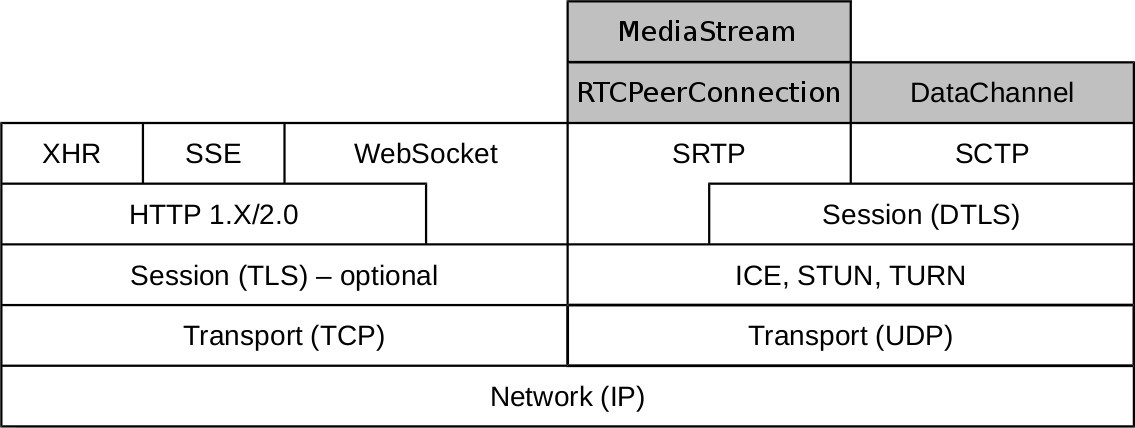
\includegraphics[width=\textwidth]{figures/webrtc_stack2.png}
			\caption{WebRTC protocol Stack}
		\end{figure}
		\end{frame}



	\subsection{Signaling: meet and get to know}
  		\begin{frame}[c]
		\frametitle{Signaling: meet and get to know}
		\begin{itemize}
		\item Own Implementation
		\vfill
		\item SIP
		\vfill
		\item XMPP
		\vfill
		\item SigOFly
		\end{itemize}
		\end{frame}



	\subsection{Hypermedia: more than words, more than images}
  		\begin{frame}[c]
		\frametitle{Hypermedia: more than words, more than images}
		\begin{itemize}
		\item \textbf{Concepts:} HyperText \& HyperMedia \& HyperCommunications
		\vfill
		\item \textbf{Implementations:} HyperCafe \& HyperHitchcock  % Detail on Demand
		\vfill
		\item \textbf{WebBrowser:} Ambulant \& SmillingWeb \& SVG
		\end{itemize}
		\end{frame}


 		\begin{frame}[c]
		\frametitle{Web-Browser plug-ins}
		\begin{figure}
			
\includegraphics[height=0.3\textheight]{figures/flash.jpg}
			
\includegraphics[height=0.3\textheight]{figures/silverlight.png}
		\end{figure}
		\end{frame}


	\subsection{Extending collaboration tools with time manipulation}
  		\begin{frame}[c]
		\frametitle{Signaling: meet and get to know}
		\begin{itemize}
		\item Streaming and Recording
		\vfill
		\item Media Types
		\vfill
		\item Recording and Streaming Interactive Media
		\vfill
		\item Collaborative Environment
		\end{itemize}
		\end{frame}


%\subsubsection{Streaming and Recording}\label{recstream}
%\subsubsection{Media Types}\label{mediatype}
%\subsubsection{Recording and Streaming Interactive Media}\label{intrecord}
%\subsubsection{Collaborative Environment}\label{collabenv}


\part{2}
\section{Proposed Architecture}\label{arch}

\begin{frame}[t,shrink]
\frametitle{Related Work} 
\tableofcontents[part=1,currentsection,hideothersubsections]
\tableofcontents[part=2,currentsection,hideothersubsections]
\end{frame}

\subsection{Modules}

	\begin{frame}[c]
		\frametitle{Modules}
		\begin{figure}[H]
			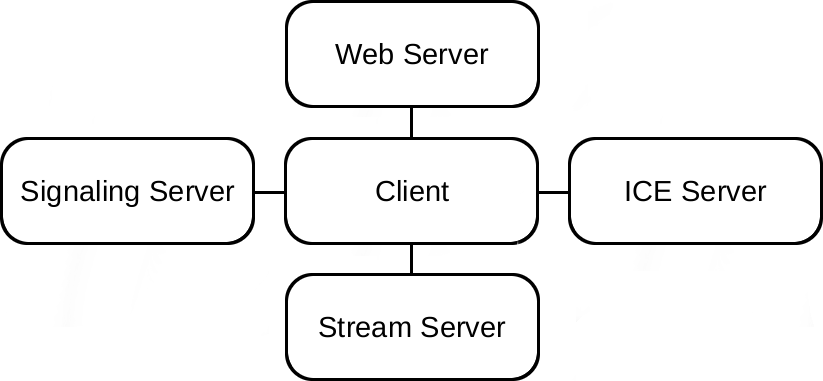
\includegraphics[width=0.6\textwidth]{figures/archs.png}
			\caption{System Modules}
		\end{figure}
	\end{frame}

\subsection{Implementation Proposal}

		\begin{frame}[c]
		\frametitle{Implementation Proposal}


\begin{columns}[c]
\begin{column}{.4\textwidth}
		\begin{figure}[H]
			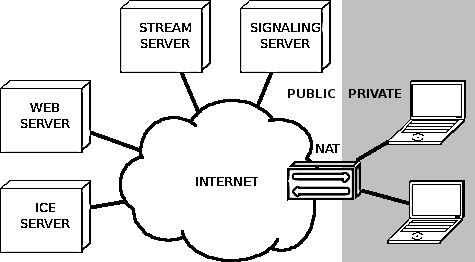
\includegraphics[width=\textwidth]{figures/arch.png}
			\caption{System Infrastructure}
		\end{figure}
\end{column}
\begin{column}{.6\textwidth}

\begin{itemize}
\small
		\item \textbf{ICE Server}: restund
		\vfill
		\item \textbf{Signaling Server}: Prosody
		\vfill
		\item \textbf{Web Server}: Play Framework
		\vfill
		\item \textbf{Stream Server}: Jitsi VideoBridge
		\end{itemize}

\end{column}
\end{columns}



{
		\centering
		\begin{figure}[H]
			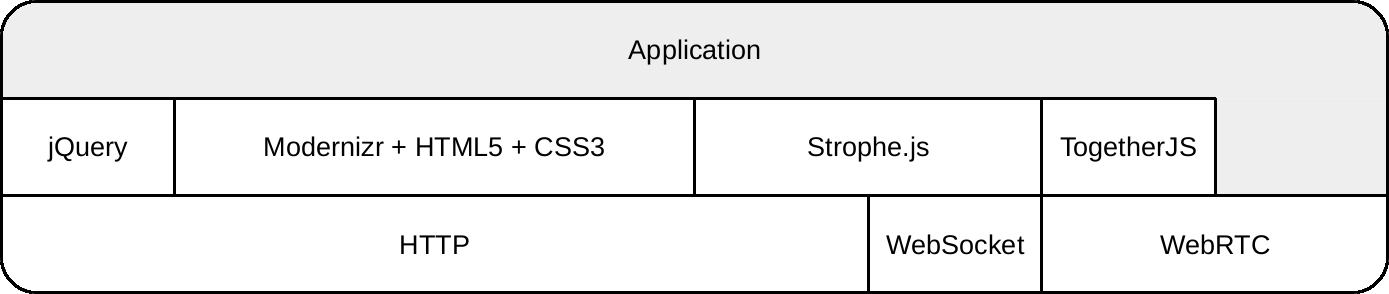
\includegraphics[width=0.8\textwidth]{figures/apparch.png}
			\caption{App Architecture}
		\end{figure}
}

		\end{frame}


\begin{frame}[c]
		\frametitle{Wireframe}
		\begin{figure}[H]
			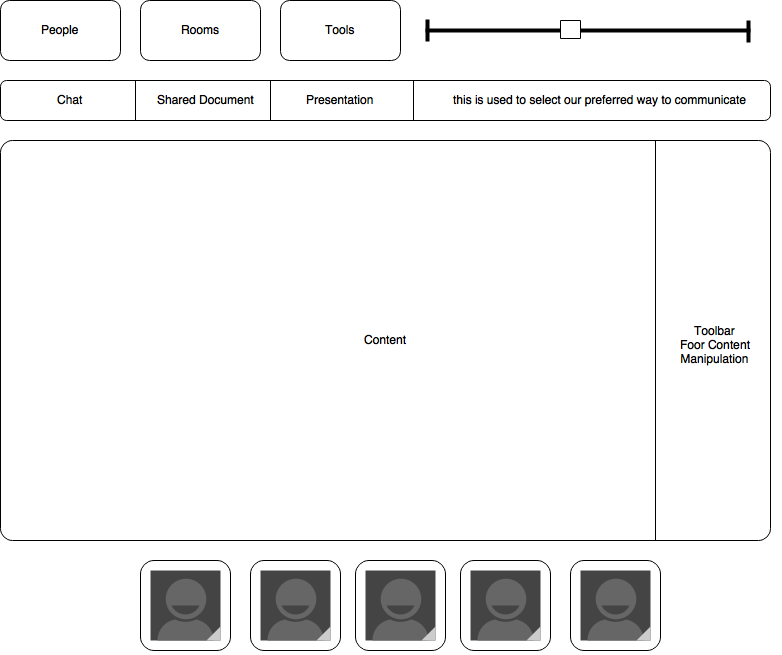
\includegraphics[width=0.6\textwidth]{figures/pbf.png}
			\caption{Application wireframe}
		\end{figure}
	\end{frame}

\section{Methodology}\label{meth} % Section

\begin{frame}[c]
		\frametitle{Methodology}
Qualitative and quantitative evaluation.

		\begin{itemize}
		\item Unit tests.
		\item Tests with users.
		\item Benchmarks.
		\end{itemize}
	\end{frame}



\subsection{Planned Schedule}
\begin{frame}[c]
\centering
		\frametitle{Planned Schedule}

\tikzset{every picture/.style={xscale=0.3,yscale=0.28,transform shape}}

\begin{ganttchart}[vgrid, hgrid]{1}{36}
\gantttitle{2015}{28}
\gantttitle{2016}{8} \\
\gantttitle{Jun}{4}
\gantttitle{Jul}{4}
\gantttitle{Aug}{4}
\gantttitle{Sep}{4}
\gantttitle{Oct}{4}
\gantttitle{Nov}{4}
\gantttitle{Dec}{4}
\gantttitle{Jan}{4}
\gantttitle{Feb}{4} \\
\gantttitlelist{1,...,36}{1}\\
%First Group
\ganttgroup{Thesis}{1}{35} \\
\ganttbar{Related work evaluation}{1}{30}\\
\ganttbar{Thesis writing}{19}{35} \\
\ganttbar{Paper writing}{25}{35} \\
\ganttmilestone{Delivery}{35}{35} \\
%\ganttlink{elem0}{elem1}
%\ganttgroup{Resume}{1}{10} \\

%\ganttmilestone{Milestone 1}{11}
%Second Group
\ganttgroup{Implementation}{1}{1}\ganttgroup{}{4}{8}\ganttgroup{}{11}{26}\ganttgroup{}{29}{30} \\
\ganttbar{Basic configuration}{1}{1} \\
%\ganttlink{elem4}{elem5}
%\ganttmilestone{Milestone 1}{11}
%Third Group
\ganttbar{WebRTC basics}{4}{4} \\
\ganttbar{Video \& Audio Communication}{4}{5} \\
\ganttbar{Non-Interactive Record \& Playback}{6}{8} \\
\ganttbar{Interactive Record \& Playback}{11}{14}\\
\ganttmilestone{First Prototype}{18}\\
\ganttbar{Collaborative Environment}{15}{18}\\
\ganttmilestone{Second Prototype}{22} \\
\ganttbar{Interface Improvement I}{19}{22} \\
\ganttbar{Usability Tests I}{23}{23} \\
\ganttmilestone{Third Prototype}{25} \\
\ganttbar{Interface Improvement II}{24}{25} \\
\ganttbar{Usability Tests II}{26}{26} \\
\ganttbar{Performance Tests}{29}{30} \\
\ganttbar{Performance Improvements}{30}{30} \\
\ganttmilestone{Final Prototype}{30}

%\ganttlink{elem8}{elem9}


\ganttlink{elem9}{elem10}
\ganttlink[link type=F-S]{elem11}{elem12}
\ganttlink{elem12}{elem13}
\ganttlink[link type=F-S]{elem13}{elem15}
\ganttlink[link type=F-S]{elem15}{elem17}
\ganttlink[link type=F-S]{elem17}{elem18}
\ganttlink[link type=F-S]{elem18}{elem20}
\ganttlink[link type=F-S]{elem20}{elem21}
\end{ganttchart}

	\end{frame}




\section{Conclusions}\label{concl} % English


\begin{frame}[c]
		\frametitle{Conclusions}

WebRTC is enabling new usage scenarios for communication and collaboration applications.
		\vfill

Theses communications will be enriched using hypermedia concepts.
		\vfill

A prototype will be implemented in order to validate these concepts.


	\end{frame}



%------------------------------------------------

%------------------------------------------------

%------------------------------------------------

\begin{frame}[c]
\Huge{\centerline{Questions?}}
\end{frame}

%----------------------------------------------------------------------------------------

\end{document} 